\documentclass[12pt,a4paper]{extreport}
\usepackage[l2tabu,orthodox]{nag}
\usepackage[left=10mm,right=50mm, top=15mm,bottom=15mm,bindingoffset=0cm]{geometry}

\usepackage{indentfirst}

\usepackage{ccaption}
\captiondelim{. }

\usepackage{amssymb,amsfonts}
\usepackage{amsmath}
\usepackage{cmap}
\usepackage{dsfont}
\usepackage[T2A]{fontenc}
\usepackage[utf8]{inputenc}
\usepackage{ucs}
\usepackage[russian,english]{babel}
\usepackage[babel = true]{microtype}
\usepackage{graphicx}
\graphicspath{{img/}}
\DeclareGraphicsExtensions{.pdf,.png,.jpg}


\usepackage{color}
\definecolor{darkblue}{rgb}{0,0,.75}
\definecolor{darkred}{rgb}{.7,0,0}
\definecolor{darkgreen}{rgb}{0,.7,0}

\usepackage[normalem]{ulem}
\usepackage[textwidth=4cm,textsize=tiny]{todonotes}
\newcommand{\fix}[2]{{\textcolor{red}{\uwave{#1}}\todo[fancyline]{#2}}}
\newcommand{\hl}[1]{{\textcolor{red}{#1}}}
\newcommand{\cmd}[1]{{\ttfamily{\textbackslash #1}}}
\usepackage[pverb-linebreak=no]{examplep}
\newcommand{\vrb}[1]{\PVerb{#1}}
\newcommand{\vrbb}[1]{\texttt{\textbackslash}\PVerb{#1}}
\newcommand{\rulez}{{\href{https://goo.gl/FhyJJm}{Правила}}}


\usepackage{listings}
    \lstnewenvironment{python}{\lstset{language=Python,
    tabsize=4,
    basicstyle=\footnotesize\ttfamily,
    stringstyle=\color{darkgreen},
    commentstyle=\color{darkred},
    keywordstyle=\color{darkblue},
    mathescape=true,
    showstringspaces=false,
    xleftmargin=.04\textwidth}}{}

\usepackage[ruled,vlined]{algorithm2e}

\usepackage[
    draft = false,
    unicode = true,
    colorlinks = true,
    allcolors = blue,
    hyperfootnotes = true
]{hyperref}

\usepackage{amsmath}

\usepackage{amsthm}
    \theoremstyle{plain}
    \newtheorem{theorem}{Теорема}
    \newtheorem{lemma}{Лемма}
    \newtheorem{proposition}{Утверждение}
    \newtheorem{corollary}{Следствие}
    \theoremstyle{definition}
    \newtheorem{definition}{Определение}
    \newtheorem{notation}{Обозначение}
    \newtheorem{example}{Пример}

\newenvironment{task}[1]
    {\par\noindent\textbf{Задача \href{http://progensys.dainiak.com/problem-#1}{#1}. }}
    {\smallskip}
\newenvironment{solution}
    {\par\noindent\textbf{Решение. }}
    {\\\bigskip}

\title{Решения задач по курсу «Дискретные структуры»}
\author{Антон Солдатенков}

\begin{document}
\maketitle

% Таким образом нужно добавлять решения задач:
\begin{task}{314}
Какое максимальное количество ребер может быть в остовном подграфе полного десятивершинного графа?
\end{task}

\begin{solution}
Клика размера 10 является остовным подграфом и содержит (по теореме о рукопожатиях) $\frac{10\cdot(10-1)}{2}=45$ ребер.
\end{solution}
\begin{task}{85}
В группе 20 студентов, из которых 5 математиков-олимпиадников, 10 обычных студентов и 5… кхм… не слишком старательных. Сколькими способами студентов можно разбить на две команды для матбоя, так, чтобы в каждой команде оказался хотя бы один олимпиадник и все не слишком старательные студенты не попали в одну команду?
\end{task}

\begin{solution}
Всего способов набрать студентов в первую команду $\frac{C^{10}_{20}}2$ (вторая команда при этом определится автоматически, разделили на 2, т. к. перестановки команд учтены дважды). Определим число случаев, не удовлетворяющих условию задачи. Во-первых, можно сформировать первую команду так, что в нее попадут все 5 олимпиадников. Тогда способов заполнить оставшиеся места в первой команде $C^{15}_5$ способов. Во-вторых, можно поместить всех раздолбаев в первую команду, тогда оставшиеся места заполняются, опять же, $C^{15}_5$ способами. В предыдущих рассуждениях два раза были учтены случаи, когда все олимпиадники находились в одной команде, а все раздолбаи в другой. Их количество $C^5_{10}$ (выберем из 10 обычных студентов 5 в первую команду). Лишний раз был учтен случай, когда все олимпиадники и раздолбаи оказались в одной команде. Всего получим $\frac{C^{10}_{20}}2 - 2 \cdot C^{15}_5 + C^5_{10} - 1$ способов.
\end{solution}
\begin{task}{62}
Вершины графа ниже занумерованы по возрастанию слева направо (номера вершин обозначены на рисунке), сверху вниз. Запишите, как этот граф будет раскрашен жадным алгоритмом. Использует ли при этом алгоритм наименьшее возможное для данного графа число цветов? Если да, то докажите, что в меньшее число цветов граф раскрасить нельзя. Если нет, то приведите новую нумерацию вершин графа, при которой алгоритм построит оптимальную раскраску.

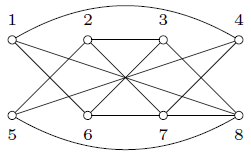
\includegraphics[width = 200pt]{img/id62.png}
\end{task}
\begin{solution}
Граф, раскрашенный жадным алгоритмом, выглядит следующим образом:

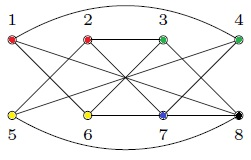
\includegraphics[width = 200pt]{img/id62_greedy.jpg}

Жадный алгоритм использует 5 цветов. Этот результат можно улучшить, перенумеровав вершины:

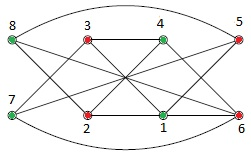
\includegraphics[width = 200pt]{img/id62_optimal.jpg}

С новой нумерацией жадный алгоритм использует всего 2 цвета.
\end{solution}
\begin{task}{58}
Назовём граф $G = (V, E)$ на $n$ вершинах $k$-критическим, если $\chi(G) = k$, и при этом при удалении любой вершины хроматическое число графа уменьшается. Докажите, что $|E|\geq n(k-1)/2$.
\end{task}
\begin{solution}
Рассмотрим произвольную вершину графа. Так как граф $k$-критический, то при удалении этой вершины хроматическое число графа уменьшается, значит, существует раскраска всех остальных вершин графа в $k - 1$ цветов. Тогда степень удаленной вершины не меньше $k-1$ (в противном случае можно было бы покрасить эту вершину в один из $k-1$ цветов, используемых при покраске оставшегося графа). Тогда суммарная степень вершин не меньше $n\cdot(k-1)$, а искомое $|E|\geq n(k-1)/2$, ч.т.д.
\end{solution}
\begin{task}{11}
На плоскости выбрано конечное количество точек, находящихся в общем положении (никакие три точки не лежат на одной прямой, никакие две не совпадают). Некоторые из выбранных точек соединены отрезками. Если два отрезка пересекаются, то их можно заменить двумя другими с концами в тех же точках (отрезки, имеющие лишь общий конец, не считаются пересекающимися). Может ли этот процесс продолжаться бесконечно? [Необходимо решить задачу непременно методом потенциалов, явно указав, какая функция используется в качестве «потенциала».]
\end{task}

\begin{solution}
Пусть $i$ -- номер итерации ($i \geq 1$). Введем функцию потенциала $f(i)$ -- суммарная длина отрезков. С каждой итерацией суммарная длина отрезков уменьшается (по неравенству треугольника), то есть $f(i+1)<f(i)$. Число различных значений этой функции конечно, так как не превосходит числа графов на $n$ вершинах ($n$ -- число выбранных точек). Значит, функция достигнет своего минимума, то есть такой процесс не может быть бесконечным.
\end{solution}
\begin{task}{32}
Приведите пример графа на 2015 вершинах, у которого ровно 1147 центральных вершин.
\end{task}
\begin{solution}
Требуемый граф состоит из клики на 1147 вершинах, к которым присоединены 868 вершин.

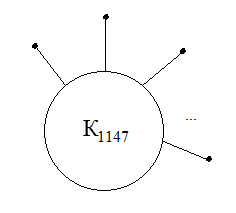
\includegraphics{img/id32.png}

Эксцентриситеты вершин клики равны 2, присоединенных вершин равны 3. Так как радиус графа равен 2, то все вершины клики являются центральными, а присоединенные ими не являются. Условие задачи выполнено.
\end{solution}
\begin{task}{66}
Планарен ли следующий граф? Если да, то нарисуйте его без самопересечений, если нет, то найдите в нём подграф, гомеоморфный $K_{3,3}$.
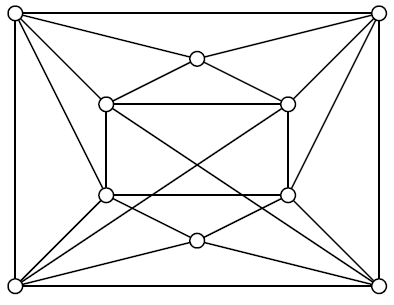
\includegraphics[width = 150pt]{img/id66.png}
\end{task}

\begin{solution}
Занумеруем вершины графа и выделим в нем подграф $K_{3,3}$ (отмечен на рисунке).

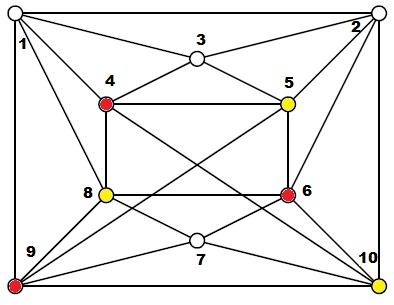
\includegraphics[width = 350pt]{img/id66_final.jpg}.

Так как граф $K_{3,3}$ гомеоморфен самому себе, то по критерию Понтрягина-Куратовского исходный граф не планарен.
\end{solution}
\begin{task}{84}Постройте троичную последовательность де Брёйна порядка два, начинающуюся с «220…». Сделайте это, найдя эйлеров цикл в соответствующем графе.
\end{task}
\begin{solution}
Построим граф де Брейна и найдем в нем эйлеров цикл (ребра в порядке обхода пронумерованы красным цветом, начальные условия учтены).
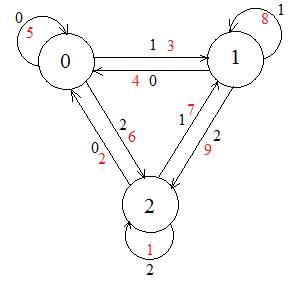
\includegraphics[width = 250pt]{img/id84.png}

Выпишем получившуюся последовательность: 2201002112.
\end{solution}
\begin{task}{143}
Найдите асимптотику величины $\binom{7n}{3n+\log_{2}{n}}$ при $n \rightarrow +\infty$. Под нахождением асимптотики понимается нахождение такой функции $f$, между которой и оцениваемой величиной можно было бы поставить знак $\sim$. Ответ принимается только в виде формулы, не содержащей неопределённостей вида $1^{\infty}, 0^0, (\text{const}+0)^{\infty}$ и пр.
\end{task}
\begin{solution}
$\binom{7n}{3n+\log_{2}{n}}=\frac{(7n)!}{(3n+\log_{2}{n})!(4n-\log_{2}{n})!}$. Используя формулу Стирлинга, получим асимптотическое равенство 
\begin{equation*}
    \begin{split}
    \binom{7n}{3n+\log_{2}{n}}\sim \frac{\sqrt{2\pi\cdot 7n}\cdot\left(\frac{7n}{e}\right)^{7n}}{\sqrt{2\pi(3n+\log_{2}{n})}\left(\frac{3n+\log_{2}{n}}{e}\right)^{3n+\log_{2}{n}}\cdot\sqrt{2\pi(4n-\log_{2}{n})}\left(\frac{4n-\log_{2}{n}}{e}\right)^{4n-\log_{2}{n}}}=\\
    =\frac{\sqrt{7n}\cdot(7n)^{7n}}{\sqrt{2\pi}\cdot\sqrt{3n+\log_{2}{n}}\cdot\sqrt{4n-\log_{2}{n}}\cdot\left(\frac{3n+\log_{2}{n}}{e}\right)^{3n+\log_{2}{n}}\cdot\left(\frac{4n-\log_{2}{n}}{e}\right)^{4n-\log_{2}{n}}}
    \end{split}
\end{equation*}
Поскольку $\log_{2}{n} = o(n)$, то последнее выражение асимптотически равно
    \begin{flalign*}
        &\sqrt{\frac{7}{24\pi}}\cdot\frac{7^{7n}\cdot n^{7n}}{\sqrt{n}\cdot(3n)^{3n+\log_{2}{n}}\cdot\left(1+\frac{\log_{2}{n}}{3n}\right)^{3n+\log_{2}{n}}\cdot(4n)^{4n-\log_{2}{n}}\cdot\left(1-\frac{\log_{2}{n}}{4n}\right)^{4n-\log_{2}{n}}}=&\\
        &=\sqrt{\frac{7}{24\pi}}\cdot\frac{7^{7n}}{\sqrt{n}\cdot3^{3n+\log_{2}{n}}\cdot 4^{4n-\log_{2}{n}}\cdot\exp\left((3n+\log_{2}{n})\cdot\ln\left(1+\frac{\log_{2}{n}}{3n}\right)\right)\cdot\exp\left((4n-\log_{2}{n})\cdot\ln\left(1-\frac{\log_{2}{n}}{4n}\right)\right)}\sim&\\
        &\sim \sqrt{\frac{7}{24\pi}}\cdot\frac{7^{7n}}{\sqrt(n)\cdot 3^{3n+\log_{2}{n}}\cdot 4^{4n-\log_{2}{n}}\cdot\exp\left((3n+\log_{2}{n})\cdot\left(\frac{\log_{2}{n}}{3n}-\frac{1}{2}\cdot\left(\frac{\log_{2}{n}}{3n}\right)^{2}+o\left(\left(\frac{\ln{n}}{n}\right)^{3}\right)\right)\right)}\cdot&\\
        &\cdot\frac{1}{\exp\left((4n-\log_{2}{n})\cdot\left(\frac{-\log_{2}{n}}{4n}-\frac{1}{2}\cdot\left(\frac{\log_{2}{n}}{4n}\right)^{2}+o\left(\left(\frac{\ln{n}}{n}\right)^{2}\right)\right)\right)}\sim&\\
        &\sim \sqrt{\frac{7}{24\pi}}\cdot\frac{7^{7n}}{\sqrt{n}\cdot 3^{3n+\log_{2}{n}}\cdot 4^{4n-\log_{2}{n}}\cdot\exp\left(\log_{2}{n}+\frac{1}{2}\cdot\frac{(\log_{2}{n})^2}{3n}+o\left(\frac{\ln{n}}{n^2}\right)\right)\cdot\exp\left(-\log_{2}{n}+\frac{1}{2}\cdot\frac{(\log_{2}{n})^2}{4n}+o\left(\frac{\ln{n}}{n}\right)\right)}\sim&\\
        &\sim \sqrt{\frac{7}{24\pi}}\cdot\frac{7^{7n}}{\sqrt{n}\cdot 3^{3n+\log_{2}{n}}\cdot 4^{4n-\log_{2}{n}}\cdot\exp\left(\frac{(\log_{2}{n})^2}{3n}+\frac{(\log_{2}{n})^2}{4n}\right)}\sim&\\
        &\sim \sqrt{\frac{7}{24\pi}}\cdot\frac{7^{7n}}{\sqrt{n}\cdot 3^{3n+\log_{2}{n}}\cdot 4^{4n-\log_{2}{n}}}
    \end{flalign*}
\end{solution}
\begin{task}{201}
Докажите, что среди любых $4^n$ натуральных чисел можно выбрать подмножество из $n$ чисел, каждая пара которых взаимно просты, либо выбрать $n$ чисел, каждая пара которых имеет общий делитель.
\end{task}
\begin{solution}
Пусть в графе вершины соединены ребрами тогда и только тогда, когда числа имеют общий делитель, больший единицы. В задаче требуется оценить сверху число Рамсея $R(n, n)$. Воспользуемся неравенством $R(s,t)\leq C_{s+t-2}^{s-1}$: $R(n,n)\leq C_{2n-2}^{n-1}$. Tак как $2^{2n-2}$ является суммой биномиальных коэффициентов, а $C_{2n-2}^{n-1}$ одним из них, то $R(n,n)\leq C_{2n-2}^{n-1}<2^{2n-2}<4^n$, что и требовалось доказать.
\end{solution}
\begin{task}{292}
Найдите количество различных ($\neq$неизоморфных!) графов на множестве вершин $\{1, 2, \ldots, 10\}$, которые состоят из трёх компонент связности, две из которых являются трёхвершинными цепями и одна — четырёхвершинным циклом?
\end{task}
\begin{solution}
Рассмотрим цепи. Число способов выбрать 3 вершины из 10 равно $C_{10}^3$, способов определить цепь из трех вершин 3 (по средней вершине). Аналогично для второй цепи вершины выбираются $C_{7}^3$ способами, цепь определяется тремя способами. Число способов определить четырехвершинный цикл $\frac{4!}{4\cdot2}=3$ (делим на 4, учитывая циклические перестановки и на 2, учитывая направление). Т. к. перестановки цепей не создают нового графа, число способов равно $\frac{C_{10}^3 \cdot C_{7}^3\cdot3^3}{2}=\frac{10!\cdot3^3}{2\cdot3!\cdot3!\cdot4!}=57600$.
\end{solution}
\begin{task}{318}
Сколько перестановок на множестве $\{1, 2, \ldots, n\}$ представимы в виде композиции чётного количества транспозиций?
\end{task}
\begin{solution}
Всего перестановок на $n$ элементах существует $n!$. Докажем, что количество четных перестановок равно количеству нечетных. Домножение (композиция) слева на цикл $(1 2)$ меняет четность перестановки, в то же время это биекция, так как при повторном домножении слева в силу ассоциативности композиции получается исходная перестановка. Утверждение доказано.
\end{solution}
\begin{task}{159}
Функция $n(s)$ задана в виде $n(s):=\max(n_0 | (n_0!)^{\ln{n_0}}\leq s)$. Найдите асимптотику этой функции при $n \rightarrow \infty$.
\end{task}

\begin{solution}
Из условия задачи $(n!)^{\ln{n}}\leq s < ((n+1)!)^{\ln(n+1)}$. Прологарифмируем полученное неравенство: $\ln{n}\cdot \ln(n!) \leq \ln{s} < \ln(n + 1)\cdot \ln((n + 1)!)$.
Докажем, что $\ln(n!) \sim n\cdot \ln{n}$.
\begin{equation*}
    \begin{split}
        n! \sim \sqrt{2\pi n}\cdot\left(\frac{n}{e}\right)^n\\
        \ln{n!} \sim n\cdot\ln{n}-n+\ln(\sqrt{2\pi n})\\
        \ln{n!} \sim n\cdot\ln{n}
    \end{split}
\end{equation*} Учитывая доказанное асимптотическое равенство, получим
\[n\cdot \ln^2{n}\lesssim \ln{s} \lesssim (n + 1)\cdot\ln^2(n + 1)\]
Так как $(n + 1)\cdot\ln^2(n + 1) \sim n\cdot \ln^2{n}$ (можно доказать, посчитав соответствующий предел), то $n\cdot \ln^2{n}\lesssim \ln{s} \lesssim n\cdot \ln^2{n}$, откуда следует, что 

\begin{equation}
\ln{s}\sim n\cdot \ln^2{n}. \label{eq:1}
\end{equation}
Прологарифмировав полученное выражение, получим:
\[\ln{\ln{s}}\sim \ln{n}+2\ln{\ln{n}}.\]
При $n\rightarrow \infty$ выполнено $\ln{\ln{n}} = o(\ln{n})$, значит, $\ln{\ln{s}}\sim \ln{n}$. Подставляя в~\eqref{eq:1}, получим асимптотику $n \sim \frac{\ln{s}}{(\ln{\ln{s}})^2}$.
\end{solution}
\begin{task}{197}
Докажите, что число неупорядоченных разбиений числа $n$, в которых ни одно слагаемое не повторяется чаще, чем 2 раза, равно числу неупорядоченных разбиений того же числа на слагаемые, ни одно из которых не делится на 3.
\end{task}
\begin{solution}
Пусть число $s$ разбивается на не делящиеся на 3 слагаемые:
\[n = (a_1 + a_1 + \ldots + a_1) + (a_2 + a_2 + \ldots + a_2) + \ldots + (a_n + a_n + \ldots + a_n) = m_1\cdot a_1 + m_2\cdot a_2 + \ldots + m_n\cdot a_n.\]
Разложим $m_1, m_2, \ldots, m_n$ по степеням тройки, получим:
\[s = \left(\sum _{j = 0}^{\infty}p_{1_j}3^j\cdot a_1 + \sum _{j = 0}^{\infty}p_{2_j}3^j\cdot a_2 + \ldots + \sum _{j = 0}^{\infty}p_{n_j}3^j\cdot a_n \right).\]
Каждый коэффициент $p_{i_j}$ не превосходит двух, все $a_i$ различны, т. к. исходные слагаемые не делились на 3. Значит, существует разбиение на повторяющиеся не более двух раз слагаемые (если $p_{i_j} > 0$, то слагаемое вычислим как $3^j\cdot a_i$, соответственно, если $p_{i_j} = 2$, то таких слагаемых будет два).
\[s = \sum _{i = 1}^{n}\sum _{j = 0}^{\infty} \sum _{k = 1}^{p_{i_j}} 3^j \cdot a_i \eqno(1).\]
Пример:
\begin{multline*}
    17=1+1+1+1+1+1+1+2+2+2+2+2=7\cdot 1+5\cdot 2= \\
    = (2\cdot 3+1)\cdot 1 + (1\cdot 3+2)\cdot 2=3+3+1+6+2+2.
\end{multline*}
Докажем, что это инъекция. Пусть имеются два различных разбиения на не делящиеся на 3 слагаемые. Значит, либо в одно из них входит $a_i$, не входящее в другое, либо множества всех $a_i$ совпадают и разбиения отличаются только коэффициентами при них. В первом случае получившиеся разбиения на слагаемые в сумме (1) будут отличаться тем самым множителем $a_i$. Во втором -- верхним пределом суммирования $p_{i_j}$.

Обратно, пусть существует разбиение на слагаемые $a_1, a_2, \ldots, a_n$, не повторяющиеся более двух раз:
$s = m_1\cdot a_1 + m_2\cdot a_2 + \ldots + m_n\cdot a_n$. Каждое слагаемое представим в виде $p_i \cdot 3^i, i \geq 0$. Сгруппируем сумму по одинаковым $p_i$ и вынесем его за скобки, тогда внутри скобок сумма степеней тройки даст коэффициент $q_i$ перед слагаемым $p_i$. Получим разложение на не делящиеся на 3 слагаемые (т. к. в исходной сумме не было более двух одинаковых слагаемых, то коэффициент при $p_i$ не будет делиться на 3).
\[s = \sum _{i = 1}^{n} \sum_{j = 1}^{q_i} p_i.\]
Пример:
\begin{multline*}
    17=3+3+1+6+2+2=1\cdot 3^1+1\cdot 3^1+1\cdot 3^0 +2\cdot 3^0+2\cdot 3^0+2\cdot 3^0=\\
    =1\cdot (3^1+3^1+3^0)+2\cdot (3^1+3^0+3^0)=1\cdot 7+2\cdot 5=1+1+1+1+1+1+1+2+2+2+2+2.
\end{multline*}
У каждого образа по построенному преобразованию существует прообраз, значит, это сюръекция. \newline
Построена биекция, значит, искомые количества разбиений равны. 
\end{solution}
\begin{task}{96}
Рассмотрим вычеты по модулю $27$. Какие значения может принимать порядок элементов по этому модулю? Для каких элементов по модулю $27$ определено понятие порядка?
\end{task}
\begin{solution}
Порядок по модулю $n$ -- наименьшее целое число $k > 0$, такое, что $a^k \equiv 1 \pmod {n}$
Порядок определен только для взаимно простых с $m$ чисел (в нашем случае, для всех $a$, не кратных $3$). Вычислим функцию Эйлера: $\varphi(27)=27-\frac{27}{3} = 18$. По теореме Эйлера $a^{18} \equiv 1 \pmod {27}$. Тогда порядок числа $a$ является делителем 18 (1, 2, 3, 6, 9, 18). Предположим противное, пусть порядок равен $p < 18$ и $p$ не является делителем 18, то есть $18 = p\cdot c + q$ ($c$ неполное частное от деления $18$ на $p$, остаток от этого деления $q$). Тогда $q < p$. Противоречие.
\end{solution} 
\begin{task}{327}
Вычислите в $\mathds{Z}_7$ значение выражения $(2017^{-1} + 2018^{-1})^{2018}\cdot 2018$.
\end{task}
\begin{solution}
Найдем обратные элементы:
\[2018^{-1} \equiv (2018-7\cdot 288)^{-1} \equiv 2^{-1} \equiv 4 \pmod{7}.\]
\[2017^{-1} \equiv (2017-7\cdot 288)^{-1} \equiv 1^{-1} \equiv 1 \pmod{7}.\]
Исходное выражение преобразуется к виду: $5^{2018}\cdot 2$. По малой теореме Ферма $5^6 \equiv 1 \pmod{7}$, значит, $5^{2016} \equiv 1 \pmod{7}$, тогда выражение принимает вид $5^2\cdot 2 = 4\cdot 2 = 1 \pmod{7}$.
\end{solution}
\begin{task}{233}
Пусть граф $G$ таков, что $||G||\geq 10\cdot|G|$, и пусть минимальная длина циклов в $G$ равняется $t$.  Соответственно, в доказательстве теоремы о числе скрещиваний мы можем использовать вместо неравенства $cr G' > ||G'||-3\cdot|G'|$ более сильное неравенство и подобрать в финале доказательства оптимальным образом вероятность $p$, получив оценку \[cr G \geq c \cdot \frac{||G||^3}{|G|^2,}\]
где $c$ -- некоторая константа. Запишите, как константа $c$ выражается через $t$.
\end{task}

\begin{solution}
Для планарного графа с длиной минимального цикла $t$ выполнено $||G|| \leq \frac{t}{t-2}(|G|-2)$. Рассмотрим $G'$ -- изображение графа $G$ без пересечений (удалены некоторые ребра). Тогда 
\begin{flalign*}
&||G'|| = ||G|| - \text{\#удаленных ребер} \geq ||G|| - cr G. &\\
&||G|| - cr G \leq \frac{t}{t-2}(|G|-2)<\frac{t}{t-2}\cdot|G|.&
\end{flalign*}
Следовательно, $cr G > ||G|| -- \frac{t}{t-2}\cdot |G|$. Аналогично доказательству теоремы о числе скрещиваний (здесь и далее $T$ - изображение $G$ с $cr G$ скрещиваниями, $G'$ -- подграф, порожденный выбранным множеством вершин),
\begin{flalign*}
&\mathds{E}(|G'|) = |G|\cdot p &\\
&\mathds{E}(||G'||) = ||G||\cdot p^2 &\\
&\mathds{E}(\text{\#скрещиваний в } T') = cr G \cdot p^4.&
\end{flalign*}
Поскольку (из доказательства) $\mathds{E}(\text{\#скрещиваний в } T')>\mathds{E}(||G'||)-\frac{t}{t-2}\mathds{E}(|G'|)$, то \newline $cr G \cdot p^4 > p^2\cdot ||G|| - p\cdot \frac{t}{t-2}\cdot |G|$. Сокращая на $p^4$, получим $cr G > \frac{||G||}{p^2}-\frac{t\cdot |G|}{(t-2)\cdot p^3}$. Возьмем производную по $p$: $-2||G||\cdotp^{-3}+3\frac{t}{t-2}|G|\cdot p^{-4} = 0$, откуда оптимальное $p = \frac32 \cdot \frac{t}{t-2}\cdot \frac{|G|}{||G||}$. Тогда искомая константа $c = \frac{4}{27}\cdot \left(\frac{t-2}{t}\right)^2$.
\end{solution}
\begin{task}{241}
Дано семейство различных $k$-элементных подмножеств $\mathcal{S} = \{A_1, A_2, \ldots A_m\}$ множества $\{v_1, \ldots, v_n\}$. Назовём элементы $v_i$ и $v_j$ соседями, если они вместе входят хотя бы в одно из множеств $A_k$. Пусть у каждого из элементов $v_j$ существует не более чем $2k$ соседей (включая сам $v_j$). Докажите, что элементы $v1, \ldots v_n$ при всех достаточно больших $k$ можно раскрасить пятью красками, так, чтобы никакое подмножество из $\mathcal{S}$  не было одноцветным.
\end{task}
\begin{solution}
Введем события $B_1, \ldots B_m$ -- множества $A_1, \ldots A_m$ одного цвета. Тогда вероятность каждого из этих событий $5\cdot \left(\frac{1}{5} \right)^k = \left(\frac{1}{5} \right)^{k-1}$. Независимость событий $B_1, \ldots B_m$ будем рассматривать как отсутствие в соответствующих им множествах $A_1, \ldots A_m$ одинаковых элементов. Найдем максимальное число зависимых событий для каждого фиксированного $B_i$. Для каждого из $k$ элементов из $2k$ соседей выберем $k$, сформировав при этом $d = k\cdot \binom{2k}{k}$ множеств, имеющих хотя бы один общий элемент с $B_i$. Докажем теперь существование такого $k$, что \[\mathds{P}(B_i) \leq \frac{1}{(d+1)\cdot e}.\]
Для этого представим биномиальный коэффициент формулой Стирлинга: $\binom{2k}{k} \sim \frac{2^{2k}}{\sqrt{\pi k}} = \frac{4^{k}}{\sqrt{\pi k}}$. Так как степень пятерки растет быстрее степени четверки, то такое $k$ существует. При этом выполнены условия леммы Ловаса, и, значит, $\mathds{P}(\overline{B_1}, \ldots, \overline{B_n}) > 0$, то есть искомая раскраска существует.
\end{solution}
\begin{task}{175}
Докажите, что матрицу из $\{0, 1\}^{n \times n}$, в каждой строке и столбце которой ровно $k$ единиц можно представить в виде суммы $k$ матриц, в каждой строке и столбце у которых в точности по одной единице.
\end{task}

\begin{solution}
Представим матрицу как матрицу смежности двудольного графа, в которой $A_{ij} = 1$ тогда и только тогда, когда между $i$-й вершиной первой доли и $j$-й вершиной второй есть ребро. Тогда искомое представление равносильно наличию в $k$-регулярном двудольном графе на $n$ вершинах $k$ совершенных паросочетаний, не содержащих общих ребер. Докажем по индукции. Для $k = 1$ утверждение очевидно. Пусть оно выполнено для некоторого $k = p - 1$. Докажем, что оно выполнено для $k = p$. Для этого убедимся, что в $p$-регулярном графе есть совершенное паросочетание. Возьмем произвольное множество $\mathcal{A}$ вершин из первой доли, пусть множество их соседей из второй доли -- множество $\mathcal{B}$. Так как во множестве $\mathcal{A}$ все вершины имеют степень $p$, то общее число ребер в графе $\mathcal{A} \cup \mathcal{B}$ равно $|\mathcal{A}|\cdot p$. С другой стороны, общее число ребер в $\mathcal{A} \cup \mathcal{B}$ не превосходит $|\mathcal{B}|\cdot p$ (так как степень каждой вершины из $\mathcal{B}$ не более $p$). Значит, $|\mathcal{B}| \geq |\mathcal{A}|$. Тогда выполнены условия теоремы Холла, а значит, в графе есть искомое совершенное паросочетание. Удалим из графа ребра, составляющие это паросочетание. Тогда останется $(p - 1)$-регулярный двудольный граф, в котором по предположению индукции существует $p - 1$ совершенных паросочетаний. Значит, в $p$-регулярном графе существует $p$ не пересекающихся по ребрам совершенных паросочетаний. Утверждение индукции доказано.
\end{solution}
\begin{task}{339}
Обозначим через $G_{s, t}$ граф на $s \cdot t$ вершинах, имеющий наибольшее число рёбер среди всех графов с кликовым числом $t$. Найдите асимптотику количества раскрасок (необязательно правильных) в $k$ цветов графа $G_{s, t}$ при $k \rightarrow \infty$.
\end{task}

\begin{solution}
Согласно теореме Турана, максимальное число ребер будет в полном $t$-дольном графе, в котором все доли имеют мощность $s$. Введем величины: $a$ -- число автоморфизмов графа $G_{s, t}$, $r$ -- число его раскрасок. По теореме Редфилда-Пойи \[r \sim \frac{1}{a} \cdot k^{|G_{s, t}|}.\]
Автоморфизмы в графе получаются переставлением долей, а затем переставлением вершин внутри каждой доли. Таким образом, $a=t!\cdot (s!)^t$. Тогда \[r \sim \frac{1}{t!\cdot (s!)^t} \cdot k^{st}.\]
\end{solution}
\begin{task}{296}
Пусть $G$ -- простой граф, а $M$ -- паросочетание в нём. Пусть количество рёбер в $M$ равно $m$. Увеличивающим путём в графе $G$ относительно $M$ называется путь (без повторяющихся вершин), в котором рёбра через одно принадлежат $M$, причём первая и последняя вершины пути не инцидентны рёбрам $M$. Докажите, что в $G$ есть паросочетание мощности $(m + k)$ тогда и только тогда, когда в $G$ найдутся $k$ увеличивающих путей без общих вершин.
\end{task}

\begin{solution}
Необходимость. Пусть в графе имеется $k$ увеличивающих путей без общих вершин, и пусть $p \leq k$ из них содержат в сумме $q \leq m$ из $M$. Для каждого из $p$ таких путей возьмем в результирующее паросочетание его нечетные ребра. Так как нечетных ребер на одно больше чем четных в каждом пути, то выбранное таким образом множество ребер имеет мощность $p + q$. Оставшиеся $k - p$ путей -- пути из одного ребра, возьмем их в результирующее паросочетание. Остались $m - q$ ребер из $M$, добавляя их, получим паросочетание мощности $(p + q) + (k - p) + (m - q) = m + k$.\newline
Достаточность. Пусть существует паросочетание мощности $(m + k)$, которое обозначим $M'$. Рассмотрим граф $G = M \cup M'$. Очевидно, все его вершины имеют степень не больше двух. Значит, все его ребра разбиваются на группы.
\begin{enumerate}
    \item 
    Одиночные.
    \begin{enumerate}
        \item 
        Принадлежащие $M$ ($p$ ребер).
        \item
        Принадлежащие $M'$ ($q$ ребер).
    \end{enumerate}
    \item 
    Совпадающие, то есть принадлежащие  $M \cap M'$.
    \item
    Цепочки.
    \begin{enumerate}
        \item Четной длины.
        \item Нечетной длины ($r$ цепочек), начинаются и заканчиваются ребрами из $M$.
        \item Нечетной длины ($s$ цепочек), начинаются и заканчиваются ребрами из $M'$.
    \end{enumerate}
    \item
    Циклы (могут быть только четной длины) ($2v$ ребер).
\end{enumerate}
Удалим из $G$ совпадающие ребра, циклы и цепочки четной длины. Тогда разность мощности множеств $M$ и $M'$ равна $k = q - p + s - r \leq q + s$. Возьмем как увеличивающие пути одиночные ребра, принадлежащие $M'$ и цепочки нечетной длины, с концами в $M'$. Они являются увеличивающими путями без общих вершин, поскольку $M'$ -- паросочетание, а внутри цепочек ребра из $M$ и $M'$ чередуются. Их $q + s \geq k$, значит, утверждение доказано.
\end{solution}
\end{document}
